\documentclass[12pt,letterpaper]{article}
\usepackage[papersize={8.5in,11in}]{geometry}
\usepackage{fullpage}
\usepackage{gensymb}
\usepackage[utf8]{inputenc}
\usepackage{graphicx}
\usepackage{amsmath,amsfonts,mathtools,amsthm,subcaption}
\author{Jiaqi Zhu \\Amath 482, Winter 2020}
\title{G\'abor Transform}

\begin{document}
\maketitle
\begin{abstract}
The G\'abor Transform is very powerful to analyze both the time and frequency of a given signal. This project aims to analyze several music peices with G\'abor Transform. Firstly, using G\'abor Transform, we create the spectrogram which allows us to visualize the frequency at each point of certain time and examine the effects of each G\'abor Transform parameter on the spectrogram. For the second part, we use G\'abor Transform to reproduce the music score and compare the piano and recorder based on their spectrogram.  
\end{abstract}

\section*{I. Introduction and Overview}
This project aims to analyze several music peices with time-frequency analysis by using G\'abor Transform. It consists of two parts. 
\\For the first part, I will analyze a 9-s music peice by using the G\'abor filtering to produce the spectrogram. Then, I'm supposed to determing the effects of window width, translation of the G\'abor Transform and different G\'abor windows on the spectrogram. 
\\For the second part, I will analyze the song \textit{Mary had a little lamb} on both the piano and recorder. By applying G\'abor filtering, I will repoduce the music score for both music peices and determine the difference of the two instruments based on their spectrogram. 

\section*{II. Theoretical Background}
\subsection*{G\'abor Transform}
To analyze both the time and frequency property of a given signal, G\'abor D\'enes was first to propose a formal method to localize both the time and frequency. Instead of the original Fourier transform kernal, he introduced a new kernal:
$$g_{t,w}(\tau) = e^{iw\tau}g(\tau-t)$$
Futher, the G\'abor Transform is defined as:
$$G[f](t,w) = \tilde{f}_g(t,w) = \int_{-\infty}^{\infty}f(\tau)\bar{g}(\tau - t)e^{-iw\tau}d\tau = (f,\bar{g}_{t,w})$$
where the bar denotes the complex conjugate of the function. Then $(\tau - t)$ acts as a time filter to locate the signal over a specific window of time. 
\\Although the G\'abor Transform is able to locate both time and frequency property of a given signal, it's hard to acheive the balance between the accuracy of both time and frequency. Namely, the shorter the time filtering window, we've got less frequency information; however, the longer the time filtering window, we will get enough frequency information but lose the time resolution of the signal. 
\subsection*{G\'abor Window}
Wavelets are used in these transforms to highlight specific part of the signal. Wavelets, such as Gaussian and Mexican Hat are shifted across the time and mutiplied with the signal to construct a window section of the signal. With the above theory, there are three different G\'abor Window give:
$$Gaussian: g(t) = e^{-a(t-b)^2}$$
$$Mexican\:Hat\:Wavelet: g(t) = (1-a(t-b)^2)e^{-\dfrac{a(t-b)^2}{2}}$$
$$Step-function(Shannon)\:Wavelet: g(t) = \Bigg\{_{0\:otherwise}^{1\:if\:|t-b|\leq {a/2}}$$
where $b$ is the same as $\tau$ given in G\'abor Transform part, representing the location of the center; $a$ refers to the width of the window. 
\section*{III. Algorithm Implementation and Development}
\subsection*{Part One}
I will analyze the portion of Handel's Messiah with time-frequency analysis by using G\a'bor Transform. In order to do the transform, I will firstly initialize the parameter. The music data v is 8.92 which is almost 9 seconds so the length L = 9. To define the wavenumber k and apply FFT, I need an even number to be divided by 2 so I just eliminated the last data entry of the 73113 data entries in v. Then $n = 73113 - 1 = 73112$ represents the Fourier modes. Time t is given by L divided by frame per second. To capture the time resolution, I need to apply the G\'abor filtering. I firstly define the variable "tslide = 0:b:L" to represent the time interval, where b is the center of the window. Hence, the center will be changed by a distance of b for each step of the loop. For each time interval, I filtered the music data with G\'abor window and apply FFT to get the frequency information for each time window. Then I can determine the effects of window width a, translation  of the G\'abor Transform b and different G\'abor windows on the spectrogram. 
\subsection*{Part Two}
I will analyze the song \textit{Mary had a little lamb} on both the piano and recorder by using G\a'bor Transform. In order to do the transform, I will firstly initialize the parameter. The piano file is 16 sec so $L_{pia} = 16$, the recorder file is 14 sec so $L_{rec} = 14$. Luckily, we got both even data entries for both files so we can define the wavenumber k and apply FFT. For the G\a'bor Transform, I choose Gaussian window with a = 100 and b = 0.1 for to capture the time and frequency property of the given music. After obtaining the spectrogram, I could reconstuct the music score based on the frequency. Then I will compare the two spectrograms of two different instruments, piano and recorder. 

\section*{IV. Computational Results}
\subsection*{Window Width of the G\'abor Transform}
To explore the effect of window width, I keep the translation of the G\'abor Transform b = 0.1 but changed the window width a from 1 to 100. The results are shown in the following Figure 1. By comparing 1(a) and 1(b), we can see that the number of horizontal red lines decreases while a increased from 1 to 100, so we're supposed to lose much of the frequency information; however, it's much clearer to capture the time resolution. Hence, as the window width increases, we will capture much more accurate time resolution at the expense of the loss of the frequency information. In conclusion, there's a tradeoff between the time accuracy and frequency accuracy by filtering G\'abor Transform. 
\begin{figure}[ht]
\begin{subfigure}{.5\textwidth}
  \centering
  % include first image
  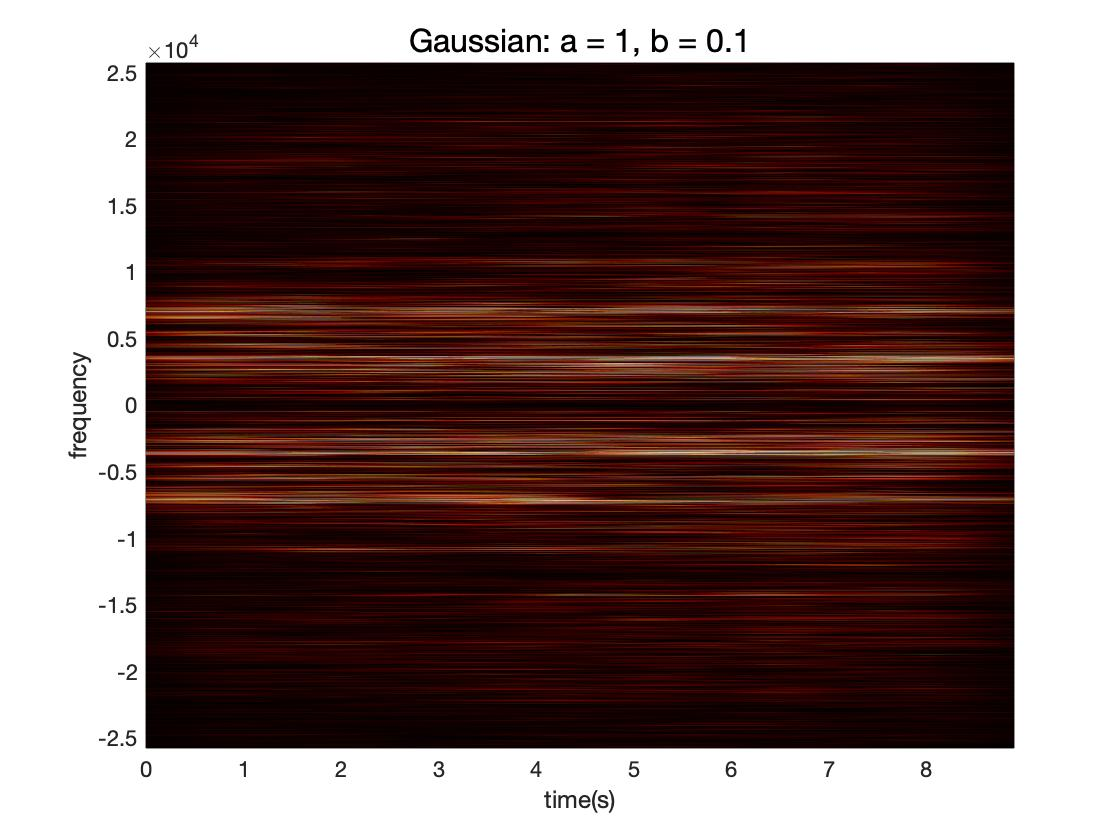
\includegraphics[width=0.8\linewidth]{1-a.jpg}  
  \caption{Gaussian: a = 1, b = 0.1}
  \label{fig:sub-first}
\end{subfigure}
\begin{subfigure}{.5\textwidth}
  \centering
  % include second image
  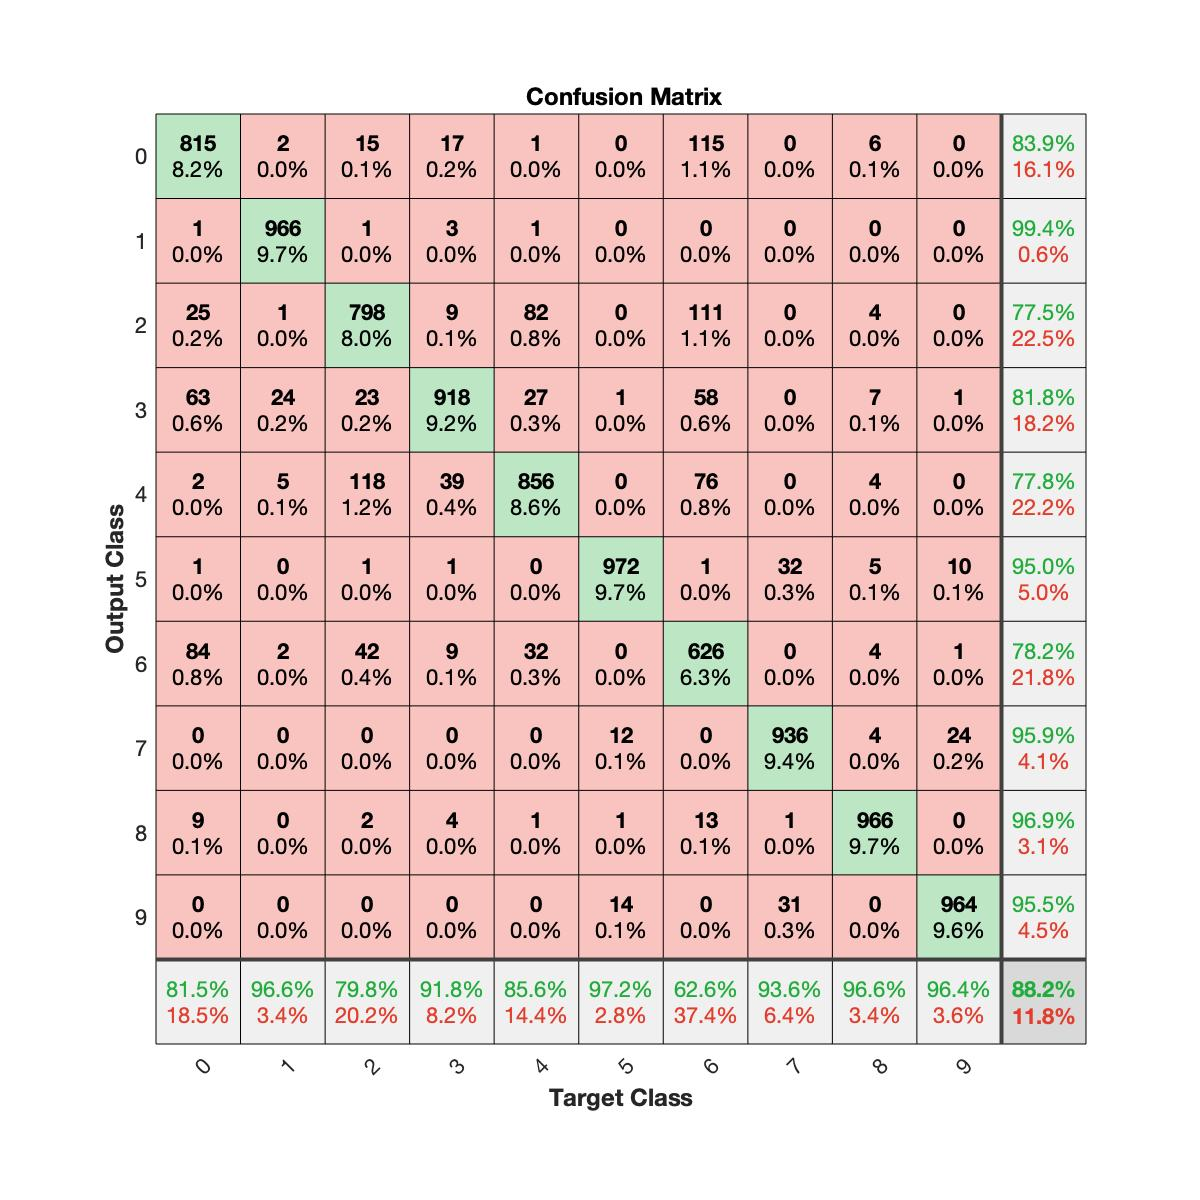
\includegraphics[width=0.8\linewidth]{1-b.jpg}  
  \caption{Gaussian: a = 100, b = 0.1}
  \label{fig:sub-second}
\end{subfigure}
\label{fig:fig}
\caption{The spectrogram of different window width}
\end{figure}

\subsection*{Oversampling and Undersampling}
To analyze the effect of the translation of the G\'abor Transform, I will keep the window width a = 10 but changed the translation b from 1 to 0.01. The results are shown in the following Figure 2. Note that smaller translation b means that we've got large number of windows which could result in oversampling. In the contrast, larger translation b means fewer number of windows which will result in undersampling. By comparing 2(a) and 2(b), we can see that the left plot is more blurry but we can have more time resolution in 2(b). Hence, undersampling provides worse time resolution but oversampling will have a better time resolution but it takes a long time. 
\begin{figure}[ht]
\begin{subfigure}{.5\textwidth}
  \centering
  % include first image
  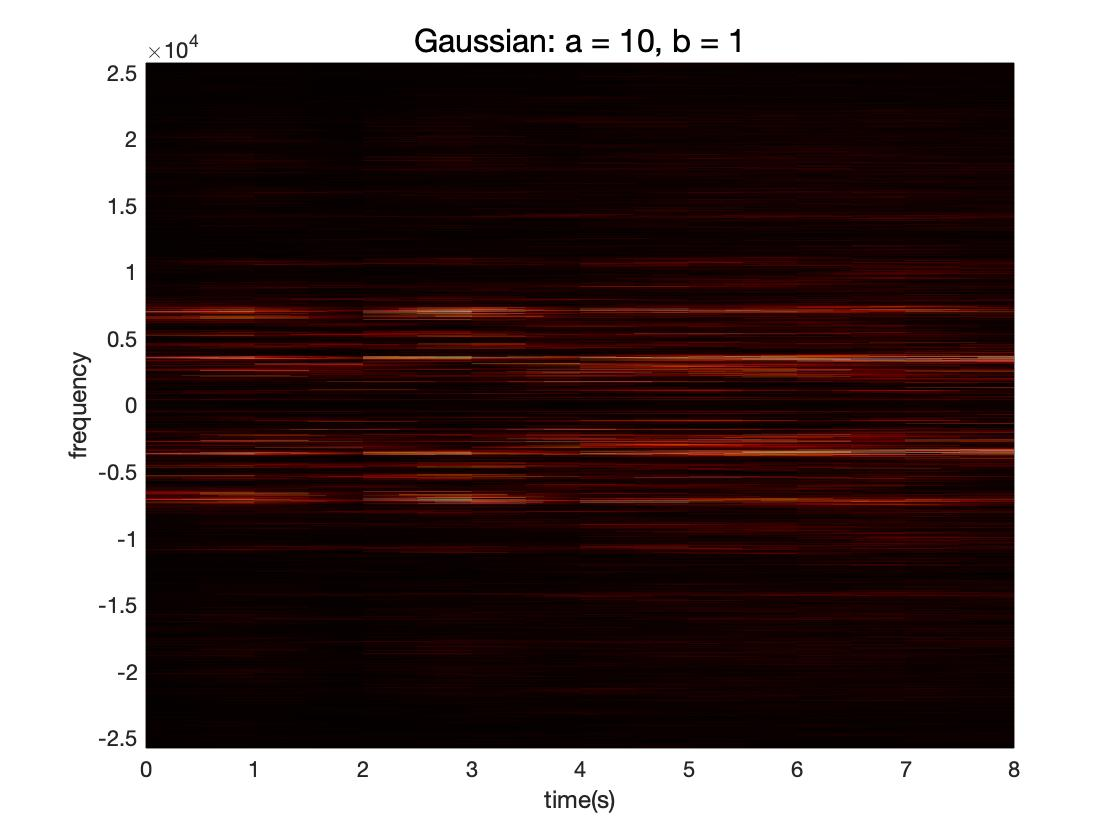
\includegraphics[width=0.8\linewidth]{1-c.jpg}  
  \caption{Gaussian: a = 10, b = 1}
  \label{fig:sub-first}
\end{subfigure}
\begin{subfigure}{.5\textwidth}
  \centering
  % include second image
  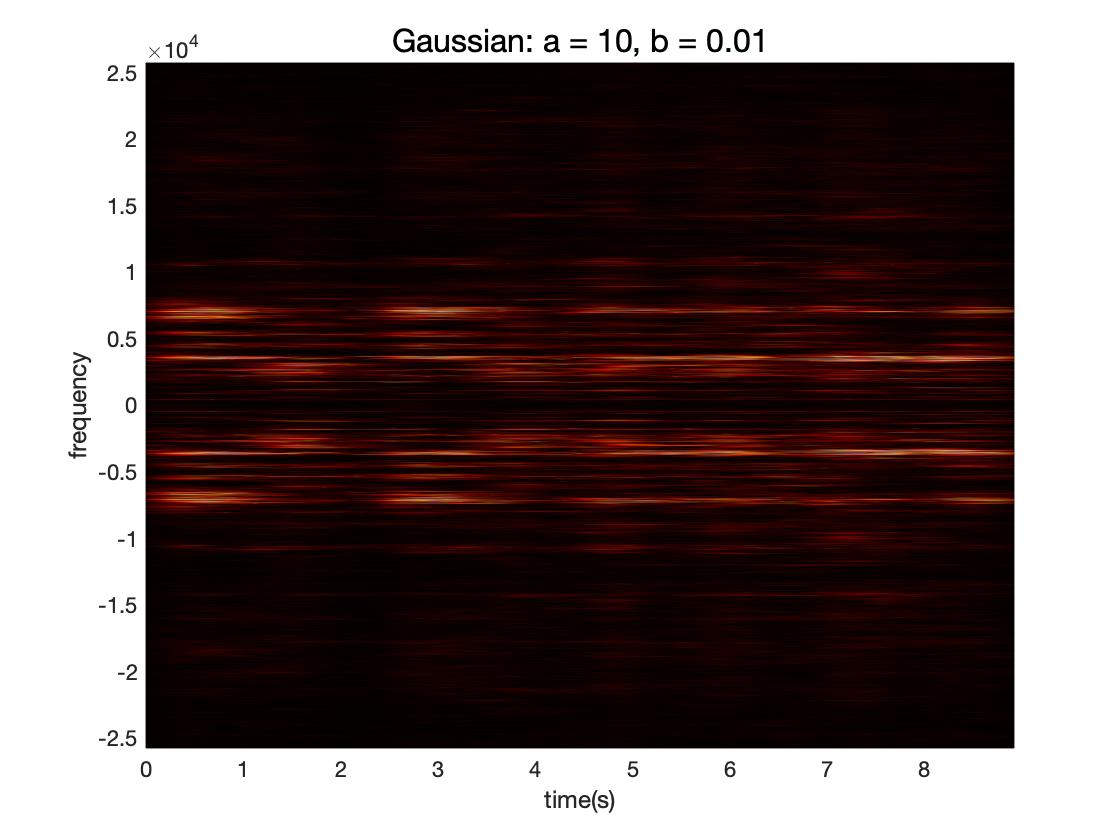
\includegraphics[width=0.8\linewidth]{1-d.jpg}  
  \caption{Gaussian: a = 10, b = 0.01}
  \label{fig:sub-second}
\end{subfigure}
\label{fig:fig}
\caption{The spectrogram of different translations}
\end{figure}

\subsection*{Different G\'abor Windows}
To compare different G\'abor Windows, I set the window width a = 100 and translation b = 0.1. The results of Gaussin is given above Figure 1(b), Mexican Hat and Step Function (Shannon) are given in the following Figure3. From the spectrogram we constructed, we can see that we will obtain the most frequency information from the Step Function wavelets because there are the most number of lines over the plot. For the rest of two, the Gaussian Filter have a better frequency resolution than the Mexican Hat. However, it means that the Mexican Hat will get the best time resolution of the three filters. There will absolutely be a tradeoff between the time accuracy and frequency accuracy by using G\'abor Transform. 
\begin{figure}[ht]
\begin{subfigure}{.5\textwidth}
  \centering
  % include first image
  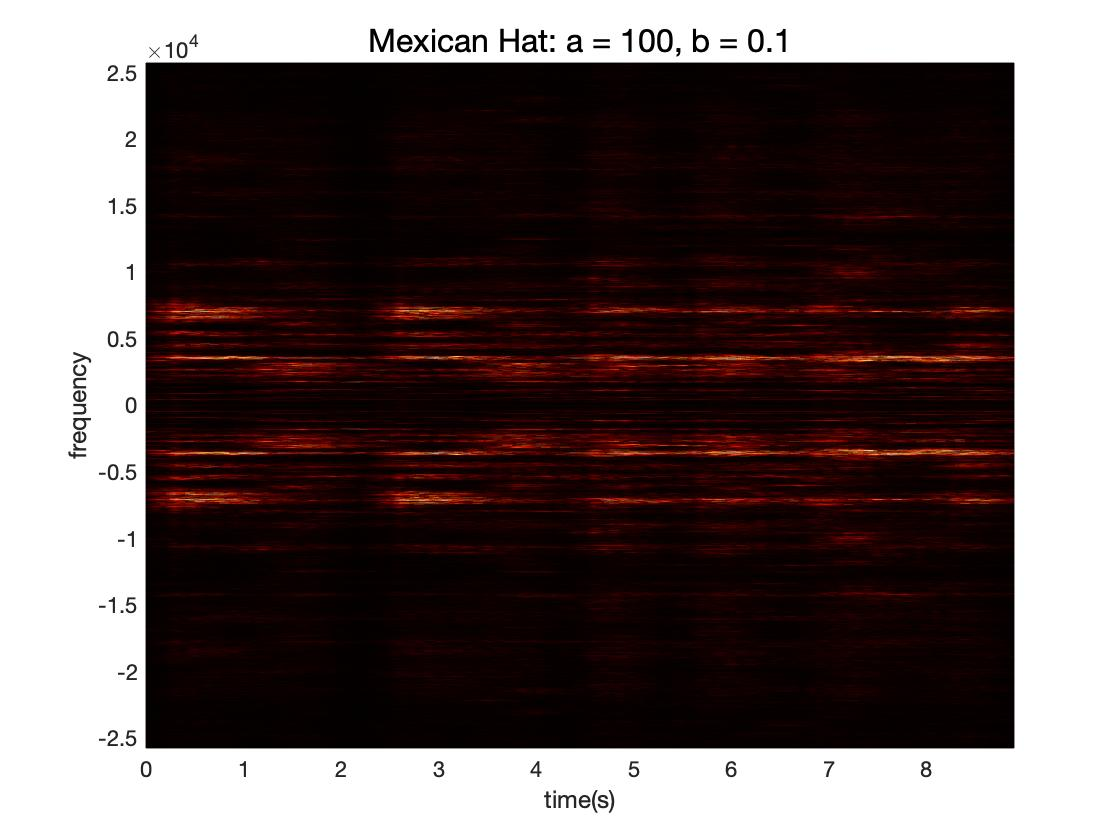
\includegraphics[width=0.8\linewidth]{3-1.jpg}  
  \caption{Mexican Hat: a = 100, b = 0.1}
  \label{fig:sub-first}
\end{subfigure}
\begin{subfigure}{.5\textwidth}
  \centering
  % include second image
  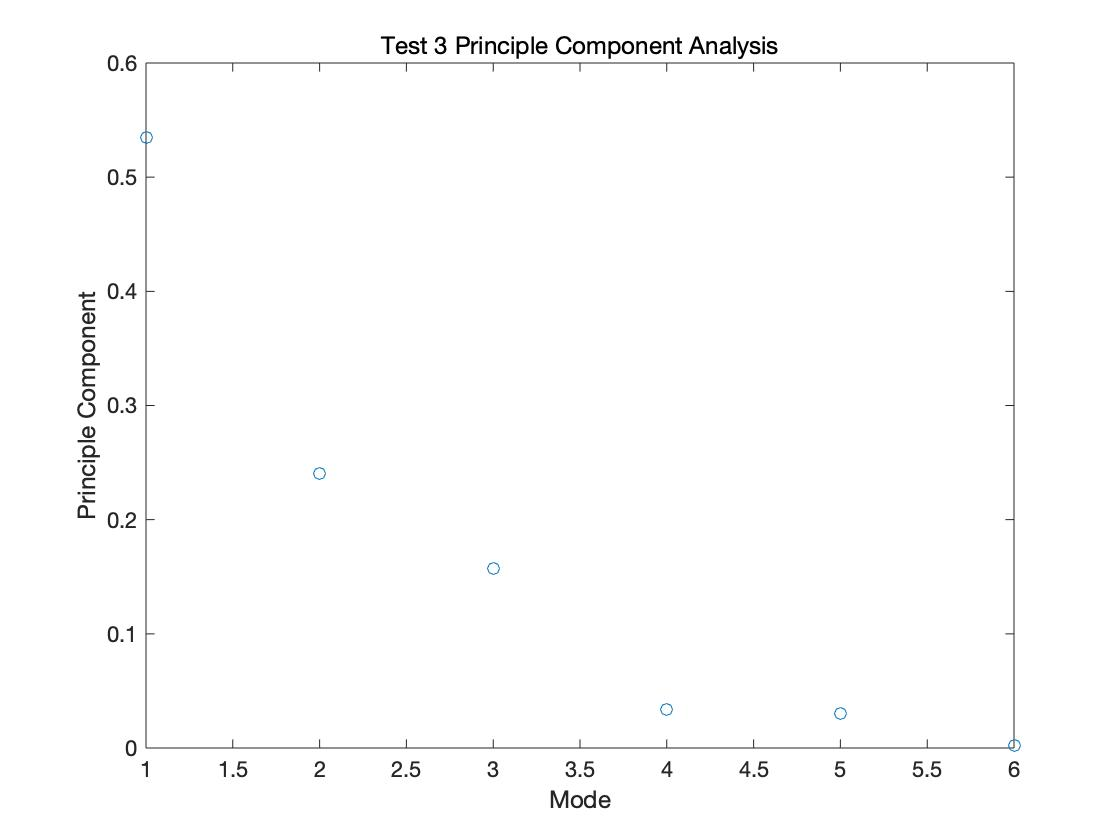
\includegraphics[width=0.8\linewidth]{3-b.jpg}  
  \caption{Step Function: a = 100, b = 0.1}
  \label{fig:sub-second}
\end{subfigure}
\label{fig:fig}
\caption{The spectrogram of different G\'abor Transform}
\end{figure}
\newpage
\subsection*{Part Two}
Through the G\'abor Transform, the spectrograms of both piano and recorder are given in the following Figure 4. Matching each frequency with the given music scale, I reconstruct the music score:
\\Piano: $E_4,D_4,C_4,D_4,E_4,E_4,E_4,D_4,D_4,D_4,E_4,E_4,E_4,E_4,D_4,C_4,D_4,E_4,E_4,E_4,
E_4,D_4,D_4,E_4,D_4,C_4$
\\Recorder:
$C_6,B_6,A_6,B_6,C_6,C_6,C_6,B_6,B_6,B_6,C_6,C_6,C_6,C_6,B_6,A_6,B_6,C_6,C_6,C_6,
C_6,B_6,B_6,C_6,B_6,G_5$
Comparing the two spectrograms, we can see that the piano file has a lower frequency than the recorder file does. Note that the definition of overtone is that if you are playing a note at frequency $w_0$, an instrument will generate overtunes at 2$w_0$, 3$w_0$,... and so far. We can see that the piano generates more overtunes. 
\begin{figure}[ht]
\begin{subfigure}{.5\textwidth}
  \centering
  % include first image
  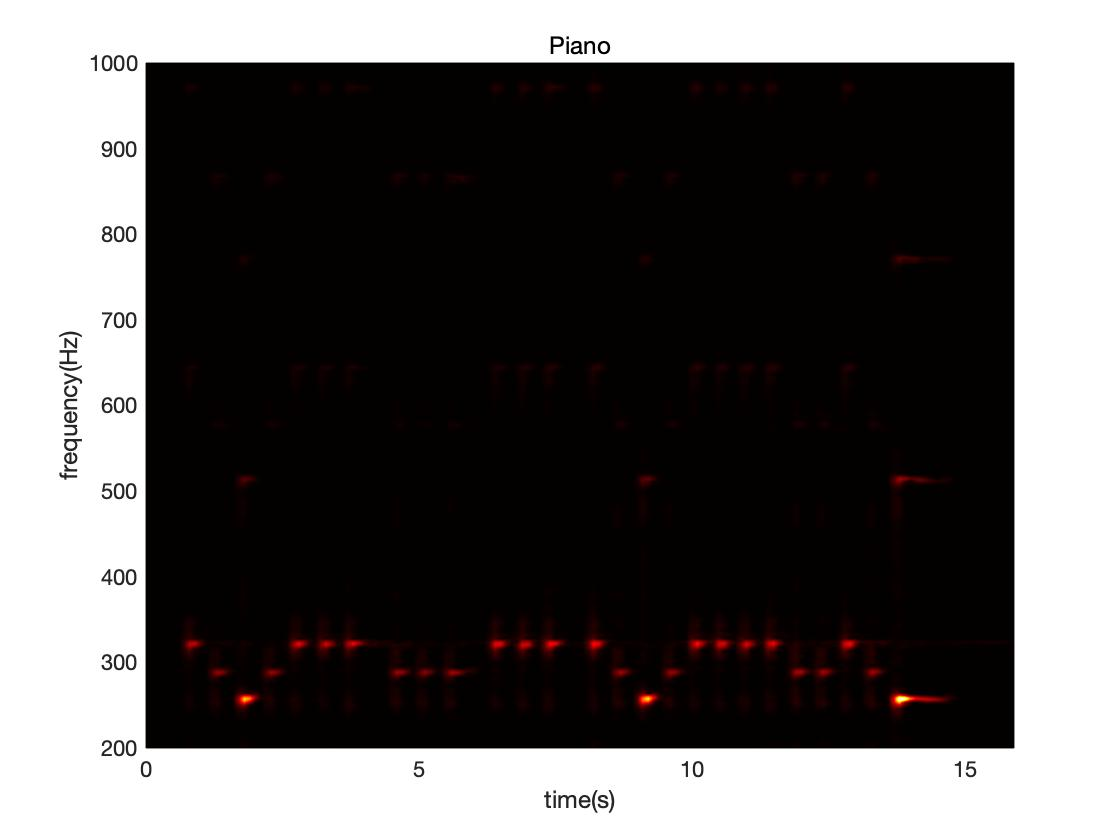
\includegraphics[width=0.8\linewidth]{4-a.jpg}  
  \caption{Piano}
  \label{fig:sub-first}
\end{subfigure}
\begin{subfigure}{.5\textwidth}
  \centering
  % include second image
  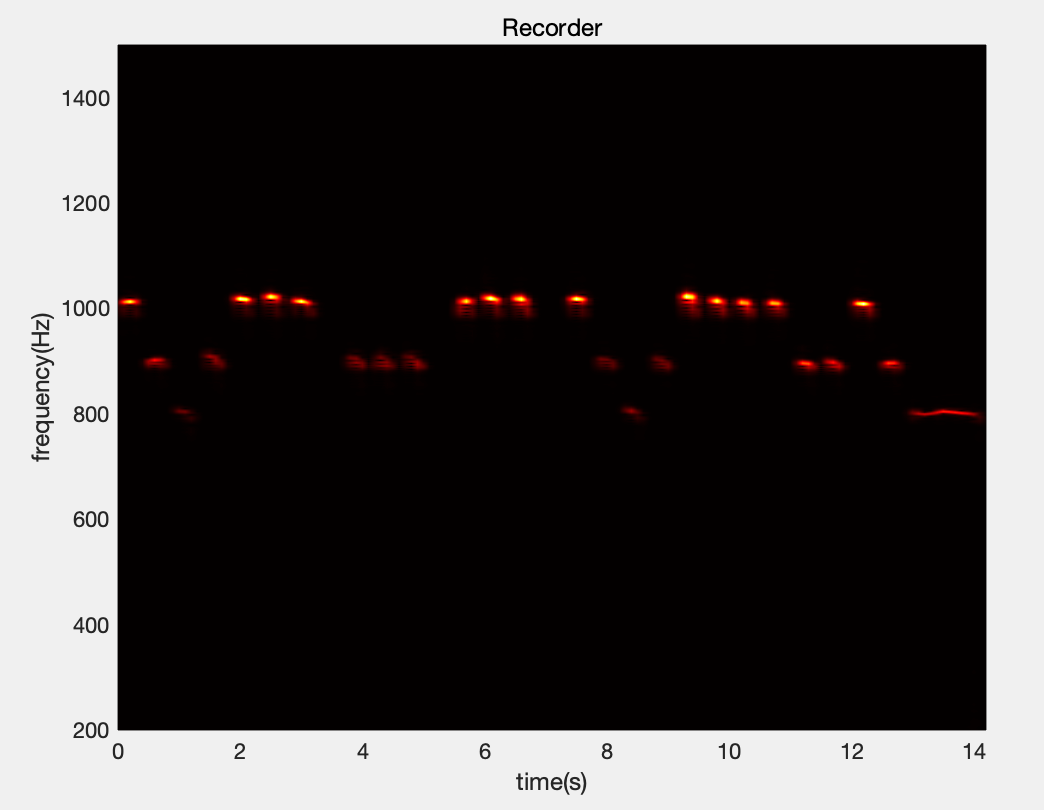
\includegraphics[width=0.8\linewidth]{4-b.png}  
  \caption{Recorder}
  \label{fig:sub-second}
\end{subfigure}
\label{fig:fig}
\caption{The spectrogram of Piano and Recorder}
\end{figure}


\section*{V. Summary and Conclusions}
For the first part of this project, I apply G\'abor Transform to obtain both time and frequency property of a portion of music. From the generated spectrogram, we find that larger window width causes a better time resolution but with a worse frequency resolution; undersampling provides worse time resolution but oversampling will have a better time resolution but it takes a long time; different G\'abor windows will shows different about time and frequency property of the music data. All in all, there'll be a tradeoff between the time accuracy and frequency accuracy. 
\\For the second part, I reconstruct the music score of the song \textit{Mary had a little lamb} on both the piano and recorder by using G\a'bor Transform. In addition, comparing the two spectrograms, we can see that the piano have more overtones. Overall, G\'abor Transform is very powerful to analyze the speech and vocalization patterns. 
\section*{Appendix A. MATLAB functions used and brief implementation explanation}
fft: fft(Sg): performs FFT on Sg.
\\
\\fftshift: fftshift(Sgt) shifts the transformed function back to its mathematically correct
positions.
\\
\\abs:  abs((fftshift(Sgt)) returns the absolute value of fftshift(Sgt). 
\\
\\pcolor(tslide, ks, $Sgt_{spec}$): draws a pseudocolor plot of matrix $Sgt_{spec}$ with x-axis tslide and y-axis ks
\\
\\shading interp: ivaries the color in each line segment and face by interpolating the colormap index or true color value across the line or face

\newpage
\section*{Appendix B. MATLAB codes}
\begin{verbatim}
clear; close all; clc; 
%% 
load handel
v = y';
v(end) = [];
%{
plot((1:length(v))/Fs;,v);
xlabel('Time [sec]');
ylabel('Amplitude');
title('Signal of Interest, v(n)');
%}

%{
p8 = audioplayer(v,Fs);
playblocking(p8);
%}

n = length(v);L = length(v)/Fs;
t = (1:length(v))/Fs;
k=(2*pi/L)*[0:n/2-1 -n/2:-1]; ks=fftshift(k);

b = 0.1;
a = 100;
Sgt_spec = [];
tslide = 0:b:L;
for j=1:length(tslide)
%g=exp(-a*(t-tslide(j)).^2); % Gabor
%g= (1-a*(t-tslide(j)).^2).*exp(-a*(t-tslide(j)).^2/2);% MH
g= abs(t - tslide(j)) <= a/2; % Shannon 
Sg=g.*v; Sgt=fft(Sg);
Sgt_spec=[Sgt_spec; abs(fftshift(Sgt))];
end

pcolor(tslide,ks,Sgt_spec.'), shading interp
title('Step Function: a = 100, b = 0.1','Fontsize',16)
xlabel('time(s)')
ylabel('frequency')
colormap(hot)

%%
%piano
[ypia,Fspia]= audioread('music1.wav');
ypia = ypia';
tr_piano=length(ypia)/Fspia; % record time in seconds
n=length(ypia);L=tr_piano;
t=(1:length(ypia))/Fspia;
k=(2*pi/L)*[0:(n/2-1) -n/2:-1]; kspia=fftshift(k);

tslide_p = 0:0.1:L;
Sgtp_spec=[];

for j=1:length(tslide_p)
%gaussian
g=exp(-100*((t-tslide_p(j)).^2));
Sgp=g.*ypia;
Sgtp=fft(Sgp);
Sgtp_spec=[Sgtp_spec; abs(fftshift(Sgtp))];
end
pcolor(tslide_p,kspia/(2*pi),Sgtp_spec'), shading interp
xlabel('time(s)');ylabel('frequency(Hz)');title('Piano')
set(gca,'Ylim',[200 1000])
colormap(hot)


%%
%record
[yrec,Fsrec] = audioread('music2.wav');
yrec = yrec';
tr_rec=length(yrec)/Fsrec; % record time in seconds
n=length(yrec);L=tr_rec;
t2=linspace(0,L,n+1); t=t2(1:n);
k=(2*pi/L)*[0:(n/2-1) -n/2:-1]; ksr=fftshift(k);

tslide_r = 0:0.1:L;
Sgtr_spec=[];

for j=1:length(tslide_r)
%gaussian
g=exp(-100*((t-tslide_r(j)).^2));
Sgr=g.*yrec;Sgtr=fft(Sgr);
Sgtr_spec=[Sgtr_spec; abs(fftshift(Sgtr))];
end

pcolor(tslide_r,ksr/(2*pi),Sgtr_spec'), shading interp
xlabel('time(s)');ylabel('frequency(Hz)');title('Recorder')
ylim([200 1500])
colormap(hot)
\end{verbatim}
\section*{Reference}
\begin{verbatim}
Kutz, Jose Nathan. Data-Driven Modeling & Scientific Computation: Methods 
	    for Complex Systems & Big Data. Oxford University Press, 2013.
\end{verbatim}
\end{document}